\documentclass[10pt]{article}

\usepackage[applemac]{inputenc}
\usepackage[english]{babel}
\usepackage[T1]{fontenc}
\usepackage{cite, url,color} % Citation numbers being automatically sorted and properly "compressed/ranged".
%\usepackage{pgfplots}
\usepackage{graphics,amsfonts}
\usepackage[pdftex]{graphicx}
\usepackage[cmex10]{amsmath}
% Also, note that the amsmath package sets \interdisplaylinepenalty to 10000
% thus preventing page breaks from occurring within multiline equations. Use:
 \interdisplaylinepenalty=2500
% after loading amsmath to restore such page breaks as IEEEtran.cls normally does.

%% Useful packages for creation of two-column and more complex figures
% Compact lists
\usepackage{enumitem}
\usepackage{booktabs}
\usepackage{fancyvrb}

\usepackage{listings} % inserisce listati di programmi
\definecolor{commenti}{rgb}{0.13,0.55,0.13}
\definecolor{stringhe}{rgb}{0.63,0.125,0.94}
\lstloadlanguages{Matlab}
\lstset{% general command to set parameter(s)
framexleftmargin=0mm,
frame=single,
keywordstyle = \color{blue},% blue keywords
identifierstyle =, % nothing happens
commentstyle = \color{commenti}, % comments
stringstyle = \ttfamily \color{stringhe}, % typewriter type for strings
showstringspaces = false, % no special string spaces
emph = {for, if, then, else, end},
emphstyle = \color{blue},
firstnumber = 1, % numero della prima linea
numbers =right, %  show number_line
numberstyle = \tiny, % style of number_line
stepnumber = 5, % one number_line after stepnumber
numbersep = 5pt,
language = {Matlab}, % per riconoscere la sintassi matlab
extendedchars = true, % per abilitare caratteri particolari
breaklines = true, % per mandare a capo le righe troppo lunghe
breakautoindent = true, % indenta le righe spezzate
breakindent = 30pt, % indenta le righe di 30pt
basicstyle=\footnotesize\ttfamily
}

%Pseudocode package
\usepackage{algorithm}
\usepackage[noend]{algpseudocode}

\usepackage{array}
% http://www.ctan.org/tex-archive/macros/latex/required/tools/
\usepackage{mdwmath}
\usepackage{mdwtab}
%mdwtab.sty	-- A complete ground-up rewrite of LaTeX's `tabular' and  `array' environments.  Has lots of advantages over
%		   the standard version, and over the version in `array.sty'.
% *** SUBFIGURE PACKAGES ***
\usepackage[tight,footnotesize]{subfigure}

\usepackage[top=2cm, bottom=2cm, right=1.6cm,left=1.6cm]{geometry}
\usepackage{indentfirst}

%\usepackage{times}
%\usepackage[active]{srcltx}

\setlength\parindent{0pt}
\linespread{1}

\def\C#1{\mathcal{#1}}

\usepackage{mathtools}
\DeclarePairedDelimiter{\ceil}{\lceil}{\rceil}
\DeclarePairedDelimiter{\floor}{\lfloor}{\rfloor}
\DeclareMathOperator*{\argmin}{arg\,min}
\DeclareMathOperator*{\argmax}{arg\,max}
%\DeclareMathOperator*{\arccos}{arc\,cos}


% Package used to keep inherent figures in the same section
\usepackage{placeins}

\graphicspath{ {images/} }



\begin{document}
\title{Network Analysis and Simulation - Homework 4}
\author{Michele Polese, 1100877}

\maketitle

\section*{Exercise 1 - A discrete event queue simulator in MATLAB}
The discrete event queue simulator is based on the simulator proposed by Law in~\cite{law}. It is a simplified version of a more general DE simulator since it has to handle just one server and the events may be only arrivals or departures. The objective is to measure the delay that users suffers when entering in the system for different utilization factors $\rho$ and for different interarrival/service times. The simulator is designed to be as more general as possible, given that the code is written in MATLAB. In particular the simulator uses the following counters:
\begin{itemize}
\item \texttt{clock} the current system time
\item \texttt{next\_arr} the time of the next arrival. It is updated whenever there is an arrival, by extracting a random interarrival time according to the specifics of the queue
\item \texttt{next\_dep} the time of the next departure. It is updated by extracting a random service time if an user arrives and finds the queue empty or if a user departs and there is at least one other user waiting in the queue. Instead, when the system is empty the \texttt{next\_dep} has no meaning and it is set to \texttt{next\_arr} + 1.
\item \texttt{time\_of\_last\_event} is the time at which the previous event happened
\item \texttt{server\_status} set to 0 if the server is free, 1 if it is busy
\item \texttt{number\_in\_queue} number of users in the queue (= number of users in the system - 1)
\item \texttt{times\_of\_arrival} a FIFO queue that collects the time of arrival of each user
\item \texttt{number\_of\_events} and \texttt{renewal\_instants} are 2 counters that could set the stopping time of the simulation. Generic simulations stop when the number of events (either arrivals or departures) has reached a given maximum. Instead, if the queue has memoryless arrivals (Poisson or Bernoulli iid), the simulator counts a renewal instant when an arrival finds the queue empty, and the simulation stops when this counter reaches a given threshold, which is lower than the maximum number of events. Indeed a renewal interval is completely representative of the statistics of the queue and since for small utilization factors $\rho$ they are short, then it is sufficient a smaller number of events than the maximum allowed. 
\end{itemize}

There's an initial phase of initialization, with the extraction of the first interarrival time (and the first departure time set to the previous plus 1), and the counters all to 0. Then at each step the simulator checks whether the next event is an arrival or a departure by comparing \texttt{next\_arr} with \texttt{next\_dep}. This explains why when the system is empty \texttt{next\_dep} is set to \texttt{next\_arr} + 1: the next event will be surely an arrival. 

If the event is an arrival, the simulator extracts the next interarrival time $t_a$ and stores \texttt{clock} + $t_a$ in \texttt{next\_arr}. It checks if the queue is empty, in this case it schedules immediately a departure for the user just arrived. If not, the user is backlogged in the queue. In both cases the arrival time is stored in \texttt{times\_of\_arrival}.

If the event is a departure, the simulators performs the following operations. At first it checks if there is someone left in the queue. If not, it sets the next departure time as at the beginning at \texttt{next\_arr} + 1, instead if a user is ready enters in service it computes a random service time. Since a user has just left, the head of the queue \texttt{times\_of\_arrival} is read and popped out. The delay for that user is computed as the difference between current clock value and its arrival time, and added to a cumulative metric $D_t$. The number of departed users $u_d$ is increased by one. 

The interarrival and service times are generated with 2 dedicated functions, that can be easily extended in order to support any kind of slotted or continuous interevent time. As for now, they can handle 
\begin{itemize}
\item Poisson arrivals/departures, with exponential interevent times 
\item Arrivals/departures with probability $b$ in each slot, i.e. interevent times are geometric of mean $1/b$
\item Interevent times of 1 or 2 slot with probability 0.5 each
\end{itemize}
The slot length can be specified.

I simulated three different scenarios, an M/M/1 queue, a M/G/1 queue with service time of length 1 or 2 slots with probability 0.5 and finally a queue with geometric arrivals and departures. The simulations are called from an external script that for each $\rho$ dynamically adjusts the number of simulations needed to reach a required confidence level on the estimation of the delay. In particular at least 2 iterations are required in order to compute a sample variance. 



\section*{Exercise 2 - Read logs and analyze data}
In this second exercise the goal was to extract a look-up table from a log file of a simulator and use it to compute some measurements on useful quantities in underwater optical communications. In particular, the log files are obtained from the simulations of the ambient light irradiance $E_0$ with the simulator HYDROLIGHT. From the 3 different dump files (each for a different value of $c \in [0.15, 0.4, 2.19]$ with $c$ the attenuation coefficient) I recovered the values of $E_0$ and the corresponding depth $z$ in meters using a \texttt{perl} script. It uses a regular expression to identify the right rows of the log and selects the columns with the desired values. In Figure~\ref{fig:e0zm} $E_0$ is plotted as a function of the depth $z$.

\begin{figure}[h!]
	\centering
	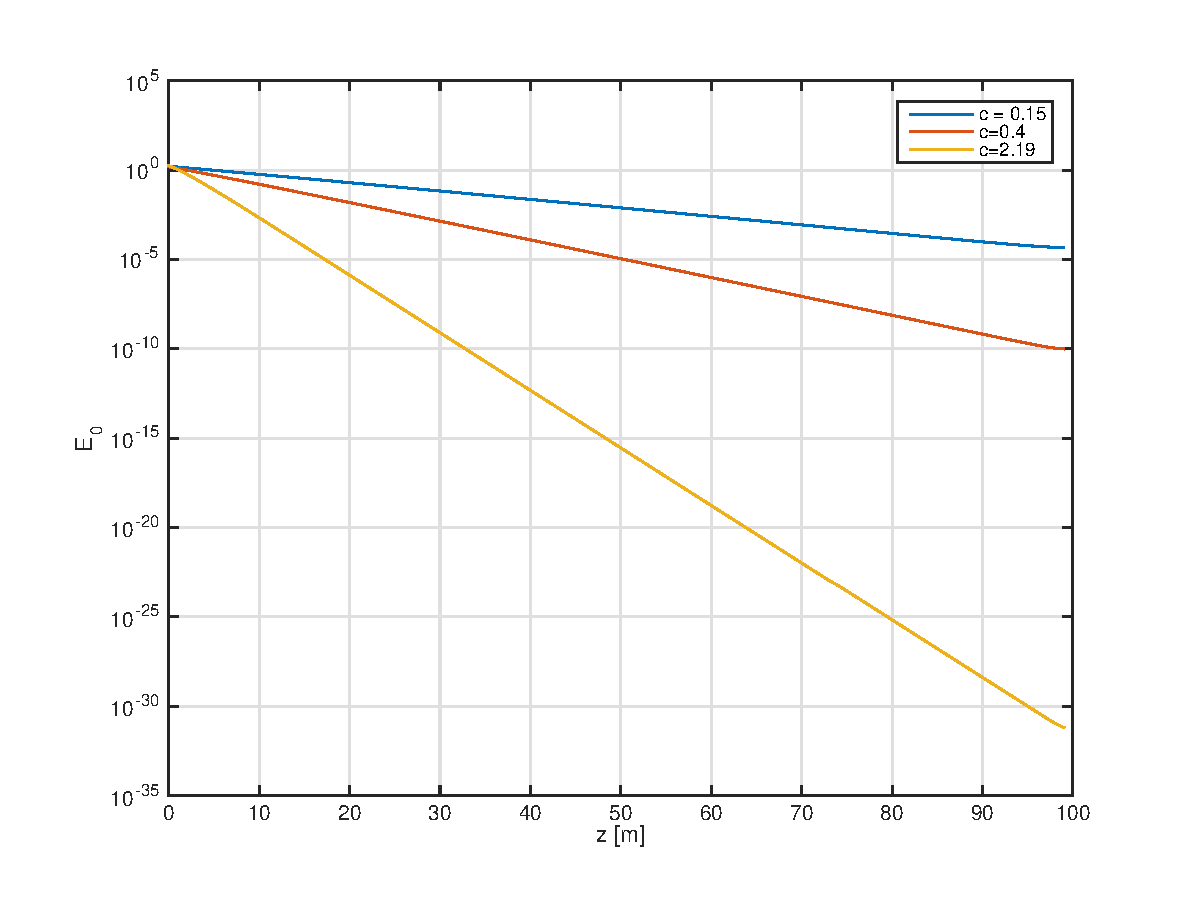
\includegraphics[width = 0.7\textwidth]{e0_z}
	\caption{Irradiance $E_0$ vs. $z$}
	\label{fig:e0zm}
\end{figure}

Some evaluation on the propagation are then carried out with a MATLAB script that uses the provided parameters for receiver and transmitter. The propagation model used the one proposed in~\cite{optmodel} and assumes that there is a successful transmission if the SNR is over a certain threshold. In particular from the irradiance and the parameters $S$ (sensitivity) and $A_r$ (area of the receiver) of the considered modem it is possible to compute the power of ambient light noise, which is $N_A = (S E_0 A_r)^2$. Let the received power $P$ be
\begin{equation}
	P = \frac{2 P_{tx} A_r \cos(\beta)}{\pi d^2 (1-\cos(\theta)) + 2 A_t}e^{-cd}
	\label{eq:p_opt}
\end{equation}
then the SNR is
\begin{equation}
	\Gamma  = \frac{(SP)^2}{2q(I_D + I_L)BW + \frac{4KTBW}{R} + N_A}
	\label{eq:snr_opt}
\end{equation}
In the following, if the SNR is above the threshold of 20 dB then there is a successful transmission. In particular, by setting the threshold and a distance $d = 10$ m, by inverting~\eqref{eq:snr_opt} in order to get $P$ and~\eqref{eq:p_opt} in order to compute $P_{tx}$ it is possible to know which is the minimum transmission power that can be used to reach a distance $d$. In Figure~\ref{fig:ptx}[a] there is the plot of the minimum $P_{tx}$ against the irradiance $E_0$, while in Figure~\ref{fig:ptx}[b] the x axis is the depth $z$ considered.

\begin{figure}[h!]
	\centering
	\subfigure[$P_{tx}$ to reach $d = 10$ m as a function of $E_0$]{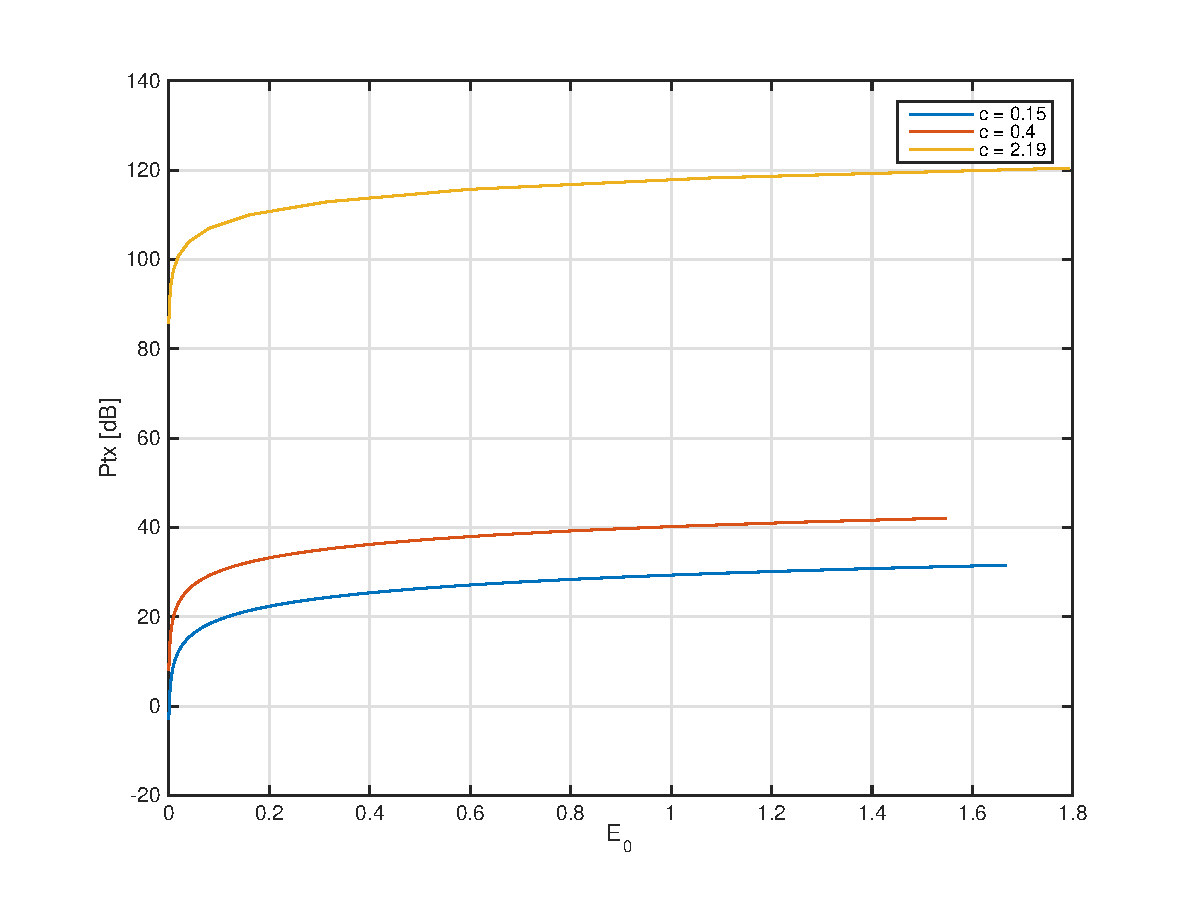
\includegraphics[width = 0.45\textwidth]{ptx_e0}}
	\subfigure[$P_{tx}$ to reach $d = 10$ m as a function of $z$]{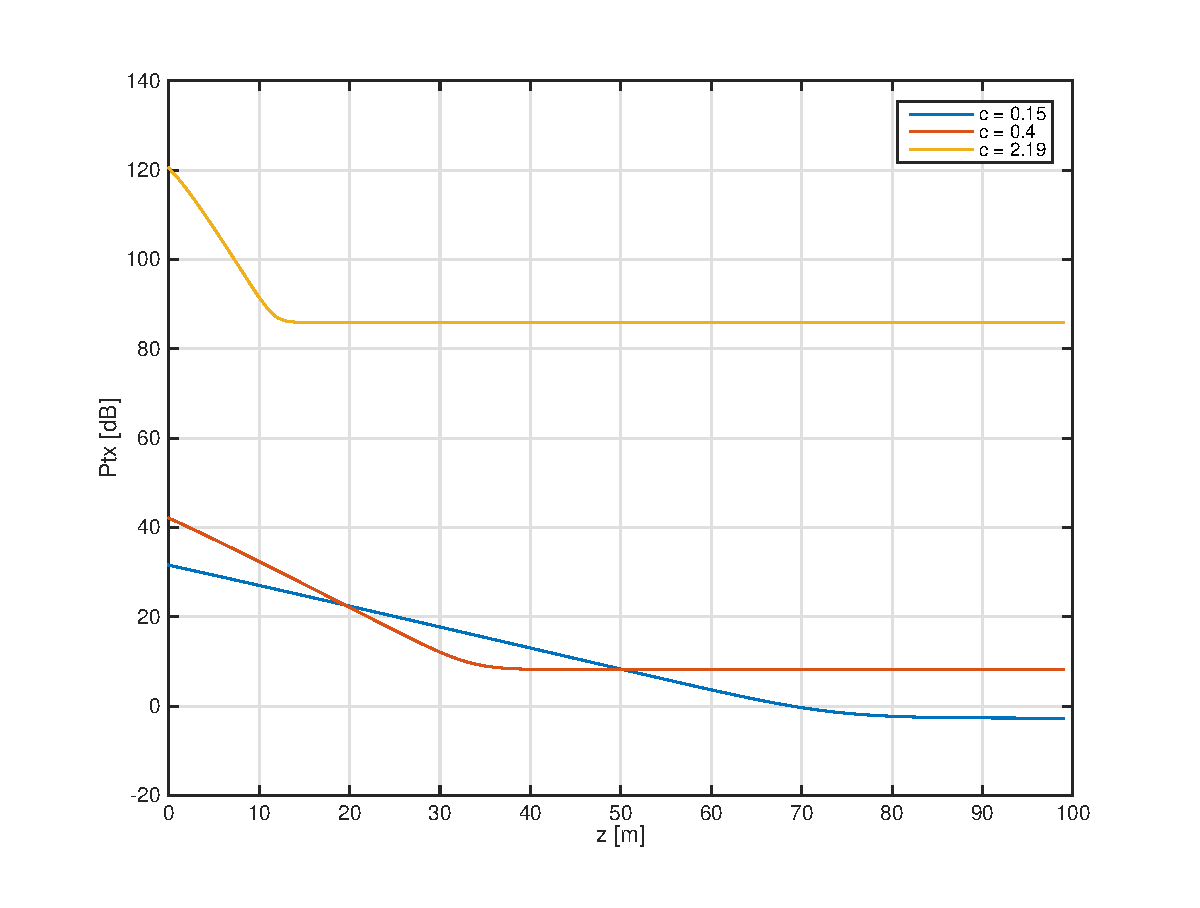
\includegraphics[width = 0.45\textwidth]{ptx_z}}
	\caption{Transmitted power $P_{tx}$ required to transmit at a distance of $d = 10$ meters}
	\label{fig:ptx}
\end{figure}

Finally, the transmit power is set to $P_{tx, max} = 100$ W and the maximum distance at which is possible to transmit is evaluated. Note that~\eqref{eq:p_opt} is not invertible with respect to the distance $d$, therefore the received power $P$ given by~\eqref{eq:p_opt} is precomputed for $d \in [0, 50]$ m and stored in a vector \texttt{P\_d}. Then, given a certain $E_0$, from~\eqref{eq:snr_opt} the minimum received power to guarantee an SNR of 20 dB is computed and the closest $P$ in \texttt{P\_d} is found. The corresponding value of $d$ is chosen as the maximum distance $d_{max}$ at which it is possible to transmit with $P_{tx, max} = 100$ W and that $E_0$ - or the corresponding $z$.

The results are in Figure~\ref{fig:dmax}.

\begin{figure}[h!]
	\centering
	\subfigure[$d_{max}$ as a function of $E_0$, for $P_{tx, max} = 100$]{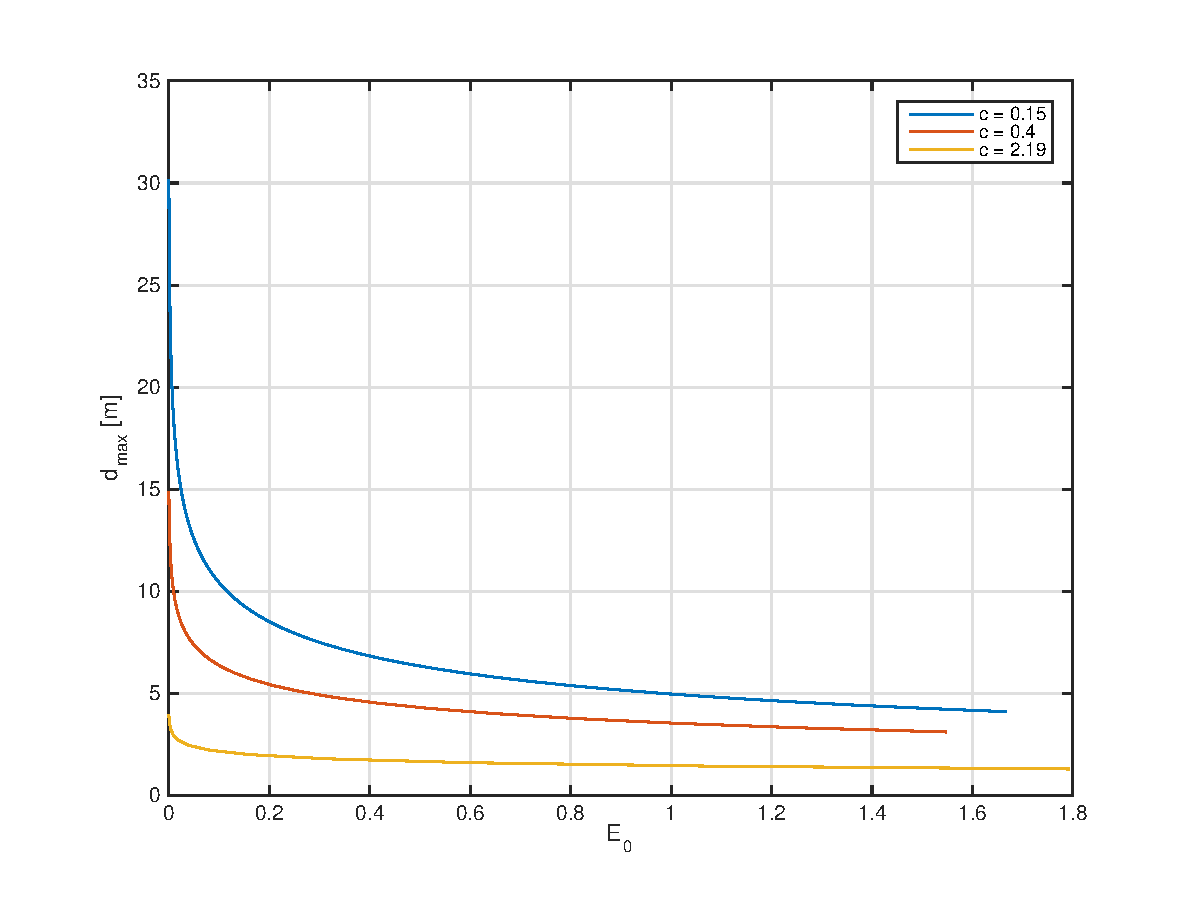
\includegraphics[width= 0.45\textwidth]{dmax_e0}}
	\subfigure[$d_{max}$ as a function of $z$, for $P_{tx, max} = 100$]{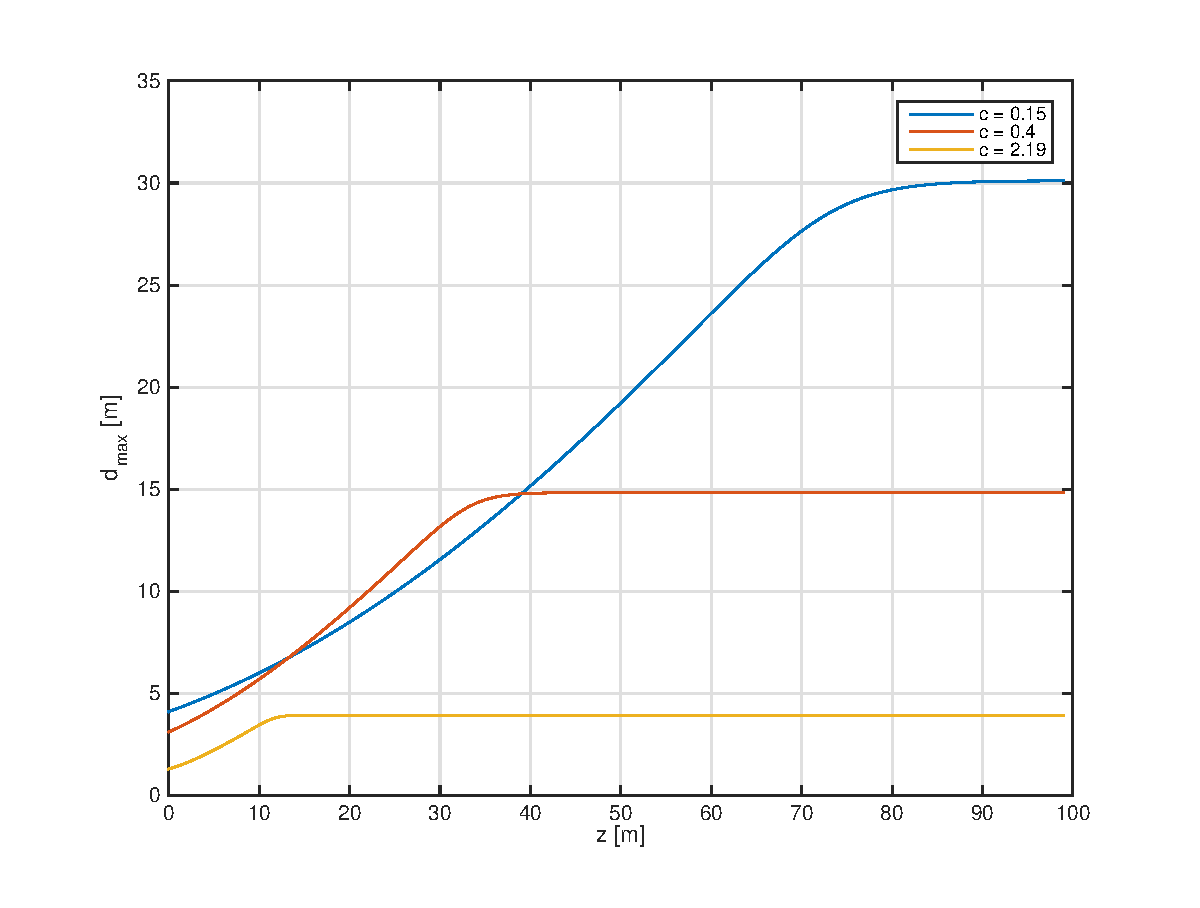
\includegraphics[width= 0.45\textwidth]{dmax_z}}
	\caption{Maximum distance $d_{max}$ with a transmit power of $P_{tx, max} = 100$}
	\label{fig:dmax}
\end{figure}


\begin{thebibliography}{10}

\bibitem{law}
A.M. Law, Simulation Modeling and Analysis, 4th ed., McGraw Hill, 2006

\bibitem{leb}
Y. Le Boudec, Performance Evaluation of Computer and Communications Systems, EPFL, 2015

\bibitem{optmodel}
D. Anguita et al., Optical wireless underwater communication for AUV: Preliminary simulation and experimental results, in Proc. IEEE/OES Oceans, Santander, Spain, Jun. 2011

\end{thebibliography}

\end{document}
